
\chapter{Homepage}

This client is fully compliant with Modbus specifications,
it allows to read and write registers through both Modbus RTU and TCP protocols.
The main window contains the basic information to configure
the protocol comunication.
A USB-485 converter is required to query RTU slaves.
Starting from version v2.38
the client implements the new standard Modbus Secure.

\begin{figure}[H]
\centering
\includegraphics[width=0.85\textwidth]{../Img/Modbus_Client_Home_00.PNG}
\caption[Homepage]{Homepage}
\end{figure}

To test the connection to an IP address use the ping button,
if the ping is successful the button colors green otherwise red.
When the connection to a slave is successful the "Running" cube is colored
green (in the case of RTU connections it is considered successful if it succeeds in 
open the selected COM port correctly).
The next part of the document will describe the various tabs and associated functions.

\newpage
\section{Modbus Secure}

Starting with version 2.38, support has been introduced for
the ModBus Secure standard, according to the specifications described 
in the document MB-TCP-Security-v21\_2018-07-24.
Flagging the checkmark "Modbus Secure" enables the "Secure" configuration 
as shown in the following image:

\begin{figure}[H]
\centering
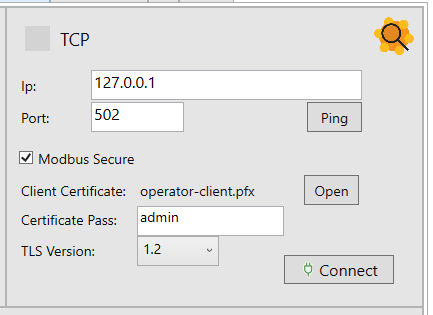
\includegraphics[width=0.6\textwidth]{../Img/ModBus_Home_Secure.PNG}
\caption[Modbus Secure]{Modbus Secure}
\end{figure}

The Modbus Secure protocol will be discussed in more detail later in section
\ref{secure}. It still works via TCP but standard datagrams are
encrypted through an SSL/TLS layer. When you check
the Modbus Secure box, a new field appears where you enter the port to be used
for secure connections, by default 802.
The Modbus Secure protocol requires (in addition to IP and port)
to load into the client
a password-protected certificate (password to be entered in the appropriate field).
The certificate should be uploaded in .pfx format, this
format contains, along with the certificate itself, also 
the private key to be used to encrypt the communication.
The client supports TLS v1.2 or 1.3 (the standard requires v1.2 or higher).
